\documentclass[10pt,a4paper]{article}
\usepackage[latin1]{inputenc}
\usepackage{amsmath}
\usepackage{microtype}
\usepackage[none]{hyphenat}
\usepackage{verbatim}
\usepackage{amsfonts}
\usepackage{amssymb}
\usepackage{enumitem}
\renewcommand{\familydefault}{\sfdefault}
\usepackage{mathpazo}
\renewcommand{\rmdefault}{put}
\usepackage{enumitem}
\usepackage[dvipsnames,svgnames]{xcolor}
\usepackage{tkz-euclide}
\usetkzobj{all}
\usepackage{graphicx}
\usepackage{tikz} 	
\usepackage{adjustbox}
\usepackage{multicol}
\usepackage{lipsum}
\usepackage[left=0.1cm,right=0.7cm,top=0.2cm,bottom=1.5cm]{geometry}
\usepackage{cancel} \usepackage{xcolor}
\usepackage{tcolorbox}
\usetikzlibrary{decorations.pathmorphing,patterns}
\usetikzlibrary{decorations.pathreplacing,calc}
 \newcommand\coret[2][red]{\renewcommand\CancelColor{\color{#1}}\cancel{#2}}

%%_------= solusi


% Set this =0 to hide, =1 to show

% Set this =0 to hide, =1 to show
\newtcolorbox{mybox}[1][] { colframe = blue!10, colback = blue!3,boxsep=0pt,left=0.2em, coltitle = blue!20!black, title = \textbf{jawab}, #1, } 


\def\showanswers{1}
\newcommand{\hide}[1]{\ifnum\showanswers=1
%
\begin{mybox}
 #1
\end{mybox}
%
\vspace{\baselineskip}\fi\ifnum\showanswers=0\vspace{2\baselineskip} \hspace{2cm}\fi}



\newcommand*\cicled[1]{\tikz[baseline=(char.base)]{\node[white, shape=circle, fill=red!80,draw,inner sep=0.5pt](char){#1};}}

\newcommand*\lingkaran[1]{\tikz[baseline=(char.base)]{\node[red, shape=circle,draw,inner sep=0.5pt](char){#1};}\stepcounter{enumii}}

\newcommand*\silang[1]{\tikz[baseline=(char.base)]{
\draw[red,thick](-0.2,-0.20)--(0.2,0.2);
\draw[red,thick](-0.2,0.20)--(0.2,-0.2);
\node[black](char){#1};
}}


\newcommand*\centang[1]{\tikz[baseline=(char.base)]{
\draw[red, very thick](-0.2,0.1)--(-0.1,0)--(0.2,0.3);
\node(char){#1};
}}

\newcommand*\merah[1]{
\textcolor{red}{#1}}
\newcommand*\pilgan[1]{
\begin{enumerate}[label=\Alph*., itemsep=0pt,topsep=0pt,leftmargin=*] #1 
\end{enumerate}}
\newcommand*\pernyataan[1]{
\begin{enumerate}[label=(\arabic*), itemsep=0pt,topsep=0pt,leftmargin=*] #1 
\end{enumerate}}



\begin{document}

\setlength{\abovedisplayskip}{0pt}
\setlength{\belowdisplayskip}{3pt}
\setlength{\abovedisplayshortskip}{0pt}
\setlength{\belowdisplayshortskip}{3pt}
%-----------------------------------------------

 \centering
  \renewcommand{\arraystretch}{2}
  \begin{tabular}{  |>{\centering\arraybackslash}m{4cm}|%
                    >{\centering\arraybackslash}m{11cm}|%
                    >{\centering\arraybackslash}m{4cm}|%
  }
    \hline
    \vspace{0.15cm} 
    \tikz[baseline=(char.base)]{
\draw[green!80!black](-0.3,-0.2) rectangle (0.3,0.2);
\node[green](char){line};
} \small{ arifstwan} &       \textbf{Ujian Nasional Fisika 2017 } 
          & arif.stwan@gmail.com 
  \\ \hline 
    
  \end{tabular}
\setlength{\columnsep}{0.2cm}
\renewcommand{\columnseprulecolor}{\color{blue!40}}

\vspace{0.15cm}

\begin{multicols*} {2} 
 \setlength{\columnseprule}{0.4pt}
\newcommand{\tikzmark}[2]{\tikz[remember picture,baseline=(#1.base)]{\node[inner sep=0pt] (#1) {#2};}} 


\begin{enumerate}[itemsep=0mm]

\item Dua buah pelat besi diukur dengan menggunakan jangka sorong, hasilnya digambarkan sebagai berikut
% Membuat jangka sorong

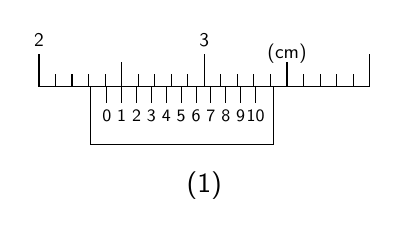
\begin{tikzpicture}[scale=2.1]
\draw[](2,0)--(4,0);
\draw (2.31,0) rectangle (3.42,-0.35);
\node at (3.5,0.2) [scale=0.7]{(cm)};
\foreach \x/\label in {2/2,3/3,4/}{ \draw (\x,0) -- (\x,0.2)node[above,scale=0.7]{\label}; } \foreach \x in {2.1,2.2,...,4}{ \draw (\x,0) -- (\x,0.075); } \foreach \x in {2.5,3.5}{ \draw (\x,0) -- (\x,0.15); }

\foreach \x [evaluate=\x as \label using \x*0.09+2.41] in {0,1,...,10}
{ \draw (\label ,0) -- (\label ,-0.1)node[below,scale=0.7]{\small{\x}}; 
}
\node at (3,-0.6) {(1)};
  \end{tikzpicture}
%
%jangka kedua
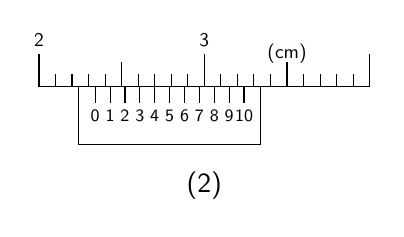
\begin{tikzpicture}[scale=2.1]
\draw[](2,0)--(4,0);
\draw (2.24,0) rectangle (3.34,-0.35);
\node at (3.5,0.2) [scale=0.7]{(cm)};
\foreach \x/\label in {2/2,3/3,4/}{ \draw (\x,0) -- (\x,0.2)node[above,scale=0.7]{\label}; } \foreach \x in {2.1,2.2,...,4}{ \draw (\x,0) -- (\x,0.075); } \foreach \x in {2.5,3.5}{ \draw (\x,0) -- (\x,0.15); }
\node at (3,-0.6) {(2)};
\foreach \x [evaluate=\x as \label using \x*0.09+2.34] in {0,1,...,10}
{ \draw (\label ,0) -- (\label ,-0.1)node[below,scale=0.7]{\small{\x}}; 
}
  \end{tikzpicture}

Selisih tebal kedua pelat besi tersebut adalah . . . 
\pilgan{
\item 0,3 mm
\item 0,6 mm
\item 0,7 mm
\item 0,8 mm
\item 1,7 mm
}



%---UN Fisika 2017-2----------
\item Sebuah benda mula-mula di titik A(0,0) kemudian bergerak selama 2 sekkon ke titik B(4,2). Selanjutnya bergerak lagi selama 3 sekon ke titik C(8,6). Kecepatan rata-rata gerak benda adalah . . . .
\pilgan{
\item {\makebox[1cm]{1 }  m.s$^{-1}$}
\item {\makebox[1cm]{1,5 } m.s$^{-1}$ }
\item {\makebox[1cm]{2} m.s$^{-1}$ }
\item {\makebox[1cm]{2$\sqrt{2}$}  m.s$^{-1}$}
\item {\makebox[1cm]{4,75 } m.s$^{-1}$}
}

%---UN Fisika 2017-3 ---------
\item Sebuah mobil mula-mula bergerak lurus dengan kecepatan konstran 72 km.jam$^{-1}$ selama 20 sekon kemudian dipercepat dengan percepatan 3 ms$^{-2}$ selama 10 sekon dan diperlambat dengan perlambatan 5 ms$^{-2}$ hingga mobil berhenti. Bentuk grafik keceptan (v) terhadap waktu (t) perjalanan mobil tersebut adalah . . . . 
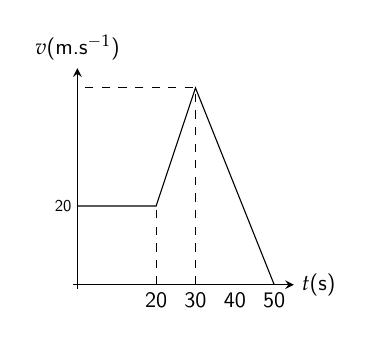
\begin{tikzpicture}[scale=0.5]
\draw[-stealth](-0.1,0)--(5.5,0) node [right,scale=0.8]{$t$(s)};
\draw[-stealth](0,-0.1) -- (0,5.5)node [above, scale=0.8] {$v$(m.s$^{-1}$)};
\draw(0,2) node [left,scale=0.6]{20}--(2,2)--(3,5)--(5,0);
\foreach \x [evaluate=\x as \label using int(\x*10)]in {2,3,4,5} {\node at (\x,0) [scale=0.8,below]{\label};}
\draw [dashed] (2,0) -- (2,2)(3,0)--(3,5)--(0,5);
\end{tikzpicture}

%----- UN Fisika 2017-4 --------
\item Perhatikan tabel data kecepatan dari tiga benda yang bergerak lurus berikut! 
\renewcommand\arraystretch{1}

\begin{tabular}{|c|c|c|c|}
\hline 
Waktu & benda A & benda B & benda C \\ \hline 
$t$(s) & $v$ (m.s$^{-1}$) &  $v$ (m.s$^{-1}$) &  $v$ (m.s$^{-1}$) \\ \hline
2 & 3 & 5 & 6 \\ \hline
4 & 14 & 9 & 10 \\ \hline
6 & 25 & 13 & 15 \\ \hline

\end{tabular}
\end{enumerate}    

\end{multicols*}
 \vspace{1cm}
%-------------------------------------------




 \end{document}
